%-----------------------------------------------------------------------------%
\chapter{\babTiga}
%-----------------------------------------------------------------------------%

%-----------------------------------------------------------------------------%
\section{Alur Penelitian}
%-----------------------------------------------------------------------------%
Dalam suatu penelitian, terdapat urutan tahapan yang perlu dilakukan. Alur penelitian ini mengandung seluruh langkah yang harus ditempuh, mulai dari fase perancangan hingga tahap akhir penelitian.
 \begin{figure}
	\begin{center}
		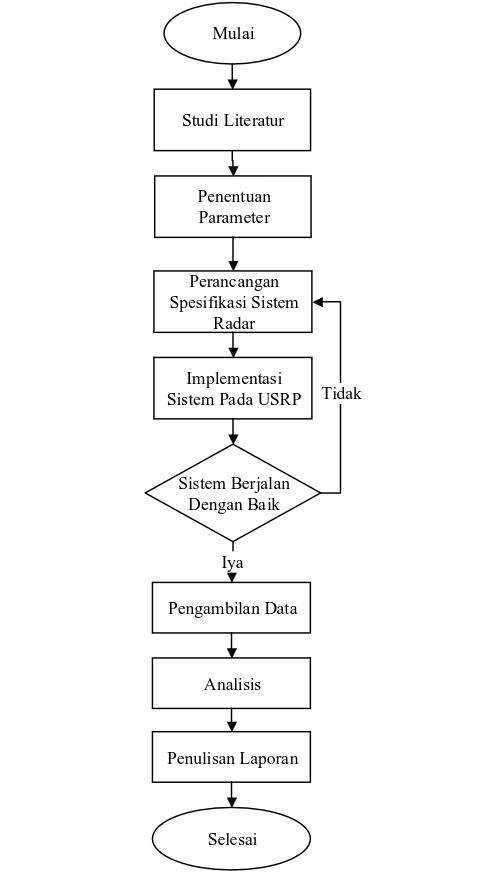
\includegraphics[scale=0.5]{pics/bab3/flowchart2.png} 
		\label{img:flowchart}
		\caption[\textit{Flowchart} Penelitian]{\textit{Flowchart} Penelitian}
	\end{center}
\end{figure}
Pada alur penelitian yang telah dirancang, terdapat 6 tahap yang perlu dilakukan setelah penelitian dimulai dan sebelum penelitian diakhiri. Tiap tahapan yang telah dirancang harus dilaksanakan sebaik mungkin agar hasil yang diharapkan dapat tercapai.


\section{Studi Literatur}
Pada tahap ini, dilakukan studi literatur terhadap masalah yang diangkat serta solusi yang diajukan pada proposal ini. Studi literatur meliputi kajian artikel terdahulu hingga kajian terhadap perangkat lunak yang digunakan serta metode yang dilakukan dalam penyelesaian masalah.
	
\section{Penentuan Parameter}

Pada tahap ini, parameter penelitian ditentukan, dengan parameter perancangan sebagai berikut.

\begin{center}
	\begin{longtable}{| c | c | c |}
		\caption{Parameter Penelitian}
		\label{tab:param}\\
		\hline
		No. & Parameter Penelitian 			& Satuan\\ \hline
		1.  &\textit{Center Frequency}	   	& GHz\\
		2.  &\textit{Bandwidth} 			& MHz \\
		\hline
	\end{longtable}
\end{center}

Sementara itu, untuk memastikan hasil yang dicapai baik, maka perlu ditentukan pula parameter pengujian, sebagai berikut.

\begin{center}
	\begin{longtable}{| c | c | c |}
		\caption{Parameter Pengujian}
		\label{tab:paramUji}\\
		\hline
		No. & Parameter Pengujian		& Satuan\\ \hline
		1.  &Jarak	   					& \\
		2.  &Kecepatan 					&  \\
		3.  &Arah						& \\
		4.  &\textit{RMSE}				&  \\
		\hline
	\end{longtable}
\end{center}

\section{Perancangan Spesifikasi Sistem}
Pada tahap ini, dilakukan perancangan tentang penelitian yang diangkat, dalam konteks ini adalah radar. Sehingga perlu dilakukannya penentuan spesifikasi radar berdasarkan perangkat keras yang digunakan. Penelitian ini menggunakan alat USRP berseri B210.  Spesifikasi dari alat ini akan dijelaskan pada tabel berikut.

\begin{center}
	\begin{longtable}{| c | c | c |}
		\caption{Spesifikasi Sistem Radar}
		\label{tab:spekRadar}\\
		\hline
		No. & Spesifikasi 					& Keterangan\\\hline
		1.  & USRP 							& B210\\
		2.  & \textit{Center Frequency}  	& 3 GHz \\
		3.  & \textit{Bandwidth} 			& A MHz \\
		4.  & Jarak Maksimum 				& A m \\
		5.  & Resolusi Jarak 				& A m \\
		6.  & Kecepatan 					& A $m/s$ \\
		7.  & Resolusi Kecepatan 			& A $m/s$\\
		\hline
	\end{longtable}
\end{center}


\section{Implementasi Sistem}
Tahap implementasi ini dilakukan pada aplikasi GNURadio dan menghasilkan \textit{flow diagram} yang merepresentasikan langkah yang dilakukan pada USRP. \textit{Flow diagram} yang didesain sudah memenuhi spesifikasi sistem radar pada tabel \ref{tab:spekRadar}.

\todo{
	Masukkan narasi simulasi sistem
}

\todo{
Detail perangkat Laptop :\\
.\\
.\\
.\\
Detail Perangkat USRP :\\
.\\
.\\
.\\
Detail Perangkat Antena \textit{Log-periodic} :\\
.\\
.\\
.\\
}

	
\section{Pengambilan Data}
Pada tahap ini, pengambilan data dengan radar yang sudah didesain dan diimplementasikan pada USRP dilakukan. Pengambilan data akan dilaksanakan di lokasi lapangan Univertitas Telkom Surabaya yang beralamat Jl. Ketintang No.156, Ketintang, Kec. Gayungan, Surabaya, Jawa Timur 60231.

\todo{Masukkan gambar peta google maps lapangan + Skenario pengujian}

\begin{figure}
	\begin{center}
		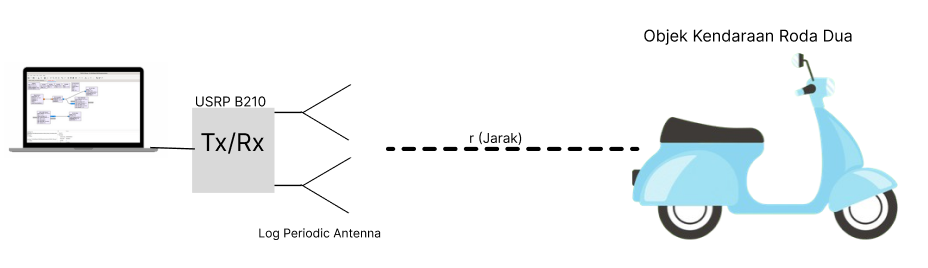
\includegraphics[scale=1]{pics/bab3/skema.png}
		\caption{Skema Penelitian}
		\label{img:skema}
	\end{center}
\end{figure}

\section{Konfigurasi Pengujian}
Konfigurasi pengujian dilakukan sesuai dengan gambar \ref{img:skema}. Terdapat satu buah perangkat laptop yang terhubung dengan dua buah USRP, masing masing USRP terhubung dengan antena \textit{Log-periodic}. USRP 1 berperan sebagai \textit{transmitter} sedangkan USRP 2 berperan sebagai \textit{receiver}.
\todo{
foto laptop + USRP + antena
}
